\documentclass[aspectratio=169]{beamer}
\usepackage{will_handley_beamer}
\usepackage{title_page}

% Commands
% --------
% - \arxiv{arxiv number}
% - \cols{width}{lh column}{rh column}
% -  \begin{fig(left|right)}[fractional width (e.g 0.6) ]{name of image}
%        content of other column
%    \end{fig(left|right)}

% Talk details
% ------------
\title{<+Title+>}
\subtitle{<+subtitle+>}
\date{<+Date+>}

\begin{document}


\begin{frame}
    \frametitle{The scaling frontier of nested sampling}
    %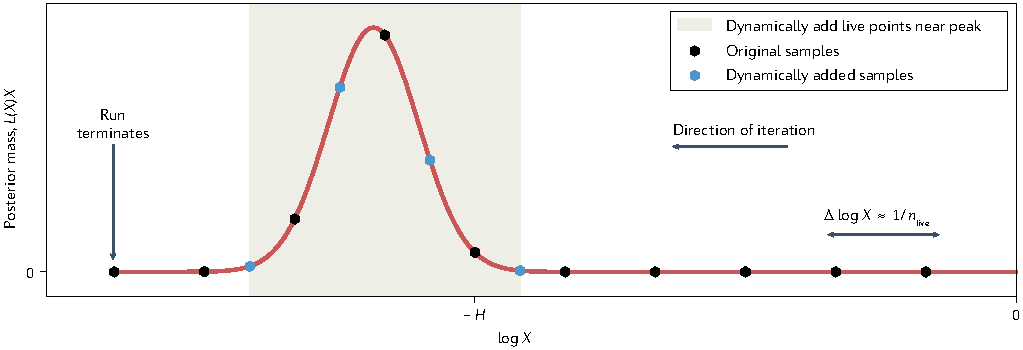
\includegraphics[width=\textwidth]{figures/run_prodecure}
    \begin{columns}[t]
        \column{0.47\textwidth}
        \begin{block}{How fast in nested sampling?}
            \[ \boxed{T = T_\mathcal{L} \times n_\mathrm{live} \times f_\mathrm{sampler} \times \mathcal{D}_\mathrm{KL}} \]
        \end{block}
        \column{0.43\textwidth}
        \begin{block}{How accurate is nested sampling?}
            \[ \boxed{\sigma \approx \sqrt{\mathcal{D}_\mathrm{KL}/n_\mathrm{live}}} \]
        \end{block}
    \end{columns}
    \vspace{10pt}
    \begin{columns}
        \column{0.5\textwidth}
        in $d$ dimensional parameter space:
        \begin{description}
            \item[$T_\mathcal{L}$:] likelihood eval time \hfill$\sim\mathcal{O}(d)$
            \item[$n_\mathrm{live}$:] number of live points\hfill$\sim\mathcal{O}(d)$
            \item[$f_\mathrm{sampler}$:] efficiency of point generation \\ region$\sim\mathcal{O}(e^{d/d_0})$ or path$\sim\mathcal{O}(d)$
            \item[$\mathcal{D}_\mathrm{KL}$:] KL between prior and posterior $\approx\log{V_\pi}/{V_\mathcal{P}}$ \hfill$\sim\mathcal{O}(d)$
        \end{description}
        \column{0.5\textwidth}
        \begin{itemize}
            \item Most attention on algorithmically improving $f_\mathrm{sampler}$, but only a fraction of the story!
            \item In my summary, will highlight where others fit into this picture
            \item $\mathcal{D}_\mathrm{KL}$ appears twice, so improvements here are quadratically important.
            \item Gradients give you $d$ more information.
        \end{itemize}
    \end{columns}

\end{frame}

\end{document}
